%!TEX root = cahier_charges_afnor.tex
\section{Présentation générale}
\subsection{Projet}
\subsubsection{Finalités}

Nous intervenons auprès d'une entreprise de développement souhaitant met\-tre à la disposition de ses clients des architectures complètes de réseaux sociaux, incluant serveur applicatif et client lourd.

\subsubsection{Espérance de retour sur investissement}

L'entreprise souhaite prendre place sur ce marché avec pour principal avantage concurrentiel de fournir des produits adaptés aux besoins précis et variés de leurs clients diffuseurs de contenu avec des délais de développement minimaux. Ces derniers attendent des progiciels fournissant des zones d'échange bien spécifiques, et expriment une forte exigence d'ergonomie.

\subsection{Contexte}

Le développement des réseaux et des moyens de communication offrent désormais beaucoup de facilité pour communiquer et échanger du contenu de nature très diverse et ceci de manière aussi très variée. Quelque soit le contenu et la manière d’organiser ces espaces de communication où l’on partage, échange des informations, leurs objectifs sont très proches.
On le voit très nettement dans l’avènement des «~réseaux sociaux~» qui les déclinent sous des formes très variées.

\subsubsection{Situation du projet par rapport aux autres projets de l’entreprise}

Notre équipe est compétente et performante en développement, notamment dans les technologies Java, et nous avons mené à bien plusieurs projets dans le cadre universitaire. Il s'agit ici de notre première réalisation commerciale.

\subsubsection{Études déjà effectuées}

L'équipe a développé au cours des années précédentes une connaissance approfondie du marché des réseaux sociaux à travers une veille technologique. Dans ce cadre, les produits facebook, MySpace, twitter, identi.ca, LinkedIn, viadeo, youtube, flickr, meetic ont été testés en profondeur.

\subsubsection{Études menées sur des sujets voisins}

Nous avons eu l'occasion de concevoir une architecture bas-niveau client-serveur pour un logiciel de gestion bibliothécaire, et de nous pencher sur le traitement et la diffusion d'informations XML à travers un serveur applicatif.

% \subsubsection{Suites prévues}

\subsubsection{Nature des prestations demandées}

L'entreprise souhaite externaliser le développement de la couche commune aux différents réseaux sociaux.

Afin de répondre au mieux aux attentes clients, l'entreprise souhaite faire développer un \emph{framework} complet et efficace, qui une fois pris en main allégera fortement les délais de développement. Pour couvrir l'ensemble des demandes et s'intégrer dans les infrastructures matérielles et logicielles hétérogènes des clients, la réutilisabilité, l'interopérabilité et la généricité de ce dernier sont fondamentales.

\subsubsection{Parties concernées par le déroulement du projet et ses résultats}

Durant toute la durée du projet, nous serons en contact avec le maître d'œuvre, M. François Puitg.

Les utilisateurs finaux seront les clients exploitant des produits développés par notre client, diffuseurs de contenu, auprès de qui nous n'interviendrons pas.

\subsection{Énoncé du besoin}

Les clients, diffuseurs de contenu, souhaitent proposer à leurs utilisateurs des zones d'échange organisées sur le modèle des réseaux sociaux~:

\begin{itemize}
	\item Gestion des relations entre les utilisateurs directement par ces derniers~;
	\item Partage facile de contenus sans structuration préalable par les équipes déployant l'architecture logicielle.
\end{itemize}

\subsection{Environnement du produit recherché}

\begin{figure}[thbp]
	\centering
		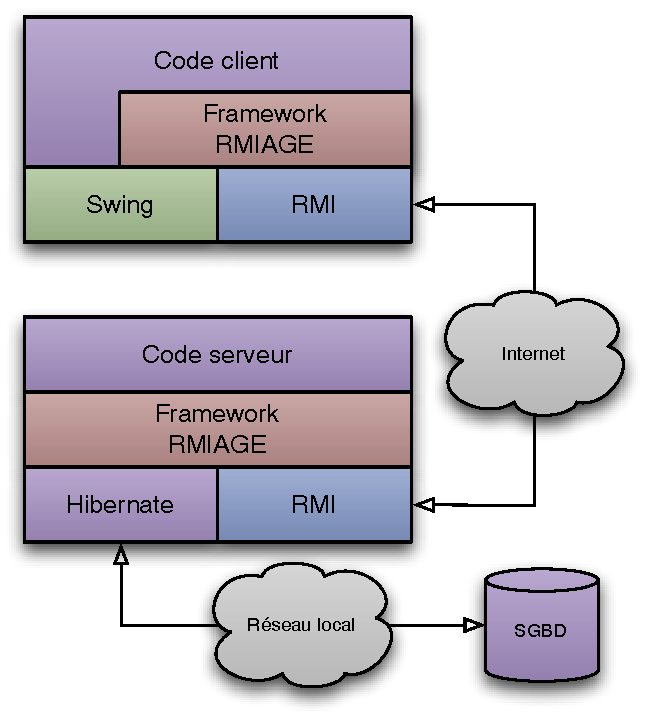
\includegraphics[scale=1]{../diagrammes/architecture.pdf}
	\caption{Architecture}
	\label{fig:archi}
\end{figure}

Le produit doit reposer sur la technologie Java, et utiliser pour la couche réseau la technologie RMI (Remote Method Invocation). L'aspect client lourd interopérable oriente vers l'utilisation de Swing. Voir figure~\ref{fig:archi}.

\subsubsection{Listes exhaustives des éléments}

Le produit se compose de trois livrables :
\begin{enumerate}
 \item Le \textit{framework} ;
 \item un programme témoin d'application serveur ;
 \item un programme témoin d'application cliente.
% \item une batterie de tests unitaires sur les fonctionnalités du framework et de l'application serveur.
\end{enumerate}

\subsubsection{Caractéristiques}
% pour chaque élément de l’environnement

\begin{enumerate}

 \item \textit{Framework}

Le \textit{framework} permettra une présentation hiérarchique des données côté client, assurant leur cohérence, et la rapidité des recherches.

Il permettra l'ajout, la suppression, la modification de celles-ci à travers une couche de sécurité conçue sur mesure pour répondre aux attentes métier.

Il fournira une application lourde très largement adaptable aux besoins et dont les composants éléments métier pourront être fournis à la volée par le serveur applicatif.

Les arborescences de contenu construites pour chaque utilisateur pourront partager des branches grâce à une gestion en graphe des données.

Des modules de gestion de contacts et de discussion seront fournis, proposant en standard des fonctionnalités fréquemment proposées sur les réseaux sociaux.

 \item Application témoin serveur
L'application témoin serveur sera une application hautement configurable, implémentant les fonctionnalités de base proposées par le serveur (modèle de sécurité minimal, démonstration d'échanges entre plusieurs clients...).

 \item Application témoin cliente

Il s'agira de l'application déployable directement par l'entreprise, et capable \emph{via} la diffusion des éléments graphiques métier par le serveur de s'adapter aux différents réseaux proposés.

Elle sera néanmoins adaptable à volonté par l'entreprise au cas par cas (ajouts de fonctionnalités, d'une documentation ad hoc, thèmes visuels, retrait du choix du serveur, implémentation/retrait de la recherche).

\end{enumerate}